\documentclass{sasbase}

\usepackage{lipsum}
\usepackage{enumitem}
\usepackage{graphicx}

\begin{document}

\title{Informationsblatt der APB}
\place{Ludwigsburg}
\datum{22. Januar 2018}
\edition{2}

\setcounter{secnumdepth}{5}

\mytitle

% OPTIONAL
%\squarestyle
% OR
\parensstyle

\section{Ankündigungen}
\begin{itemize}
    \item Am 01.02. findet die Wahl statt.
    \item Am 09.02. schließen die Bewerbungen von Richterinnen, Staatssekretärinnen und Staatsanwältinnen.
    \item In der Woche vom 19.02. bis 23.02. tagt das Parlament zum ersten Mal.
    \item Ab dem 01.03. werden Betriebsgründungen akzeptiert.
\end{itemize}
\section{Politische Bildung}
Das Informationsblatt beinhaltet auch immer FAQs zu neuen Gesetzen und der Funktionsweise der staatlichen Organe.
Fragen k\"{o}nnen gerne jederzeit an den Ausschuss f\"{u}r politische Bildung gesendet werden, diese werden so fr\"{u}h als m\"{o}gliche bearbeitet und in der n\"{a}chsten Ausgabe beantwortet.

\topic{Wahl}

\begin{question}{Wie genau läuft die Wahl ab?}
    Am Donnerstag, den 1. Februar werden eifrige Wahlhelfer in der 3./4. Stunde alle Klassen besuchen, die Wahlzettel austeilen,
    ausfüllen lassen und wieder einsammeln. Dabei werden sowohl die Präsidentin als auch die
    Parteien für das Parlament gewählt.
    \\\\
    \noindent Wer an diesem Tag \textbf{nicht} anwesend ist, hat aufgrund organisatorischer Einschränkungen \textbf{keine} andere Möglichkeit zu wählen.
    \\
    
    \noindent Sobald die Wahlzettel ausgezählt sind, werden die Wahlergebnisse per Durchsage und per
    Ankündigungsblatt durchgegeben.
\end{question}

\newpage

\begin{question}{Wer steht überhaupt zur Wahl?}
    \textbf{Parteien für die Parlamentswahl}
    \begin{itemize}
        \item Die Blauen \textbf{(DB)}
        \item Die Goethopia Partei \textbf{(DGP)}
        \item Einheitliche Arbeiterpartei \textbf{(EAP)}
        \item Frauen im Parlament \textbf{(FiP)}
        \item Goethopische Gerechtigkeitspartei \textbf{(GGP)}
        \item Kommunistisch Altruistische Partei \texbf{(KitKat)}
        \item Kleine Kätzchen Partei \textbf{(KKP)}
        \item Liberale Sozialdemokraten \textbf{(LSD)}
        \item Minderheitengremium \textbf{(MIG)}
        \item Partei für Gleichberechtigung \textbf{(PfG)}
    \end{itemize}
    
    \textbf{Präsidentschaftskandidaten}
    \begin{itemize}
        \item \textbf{Bozcali}, Aylin
        \item \textbf{Pompei}, Paula-Francesca 
        \item \textbf{Reischl}, Eric 
        \item \textbf{Schwarz}, David 
    \end{itemize}
\end{question}

\begin{question}{Wo kann ich mich informieren?}
    Um genauere Informationen über die Parteien und die Präsidentschaftskandidaten zu erhalten,
    geht einfach auf die Goethopia Webseite:
    \\\\
    \noindent\textbf{www.goethopia.de/wahl}
    \\\\
    Ihr könnt natürlich auch die Parteivorsitzenden oder Präsidentschaftskandidaten direkt
    ansprechen, um euch genauer über deren Ziele zu informieren. Darüber hinaus machen einige Parteien auch schon
    eifrig Wahlwerbung und es hängen Wahlplakate im Schulhaus aus. 
\end{question}

\begin{question}{Wie wähle ich?}
    Ein Demo-Stimmzettel hängt hier an diesem Brett aus. An sich ist das Ganze intuitiv, du machst ein Kreuz auf der linken Seite für
    den Präsidenten und ein Kreuz auf der rechten Seite für deine Partei. 
    Wenn nicht \textbf{in jeder Spalte exakt ein Kreuz ist}, ist der Wahlzettel ungültig.
    Siehe dazu auch die folgende Graphik:\\
    \begin{minipage}{0.5\linewidth}
    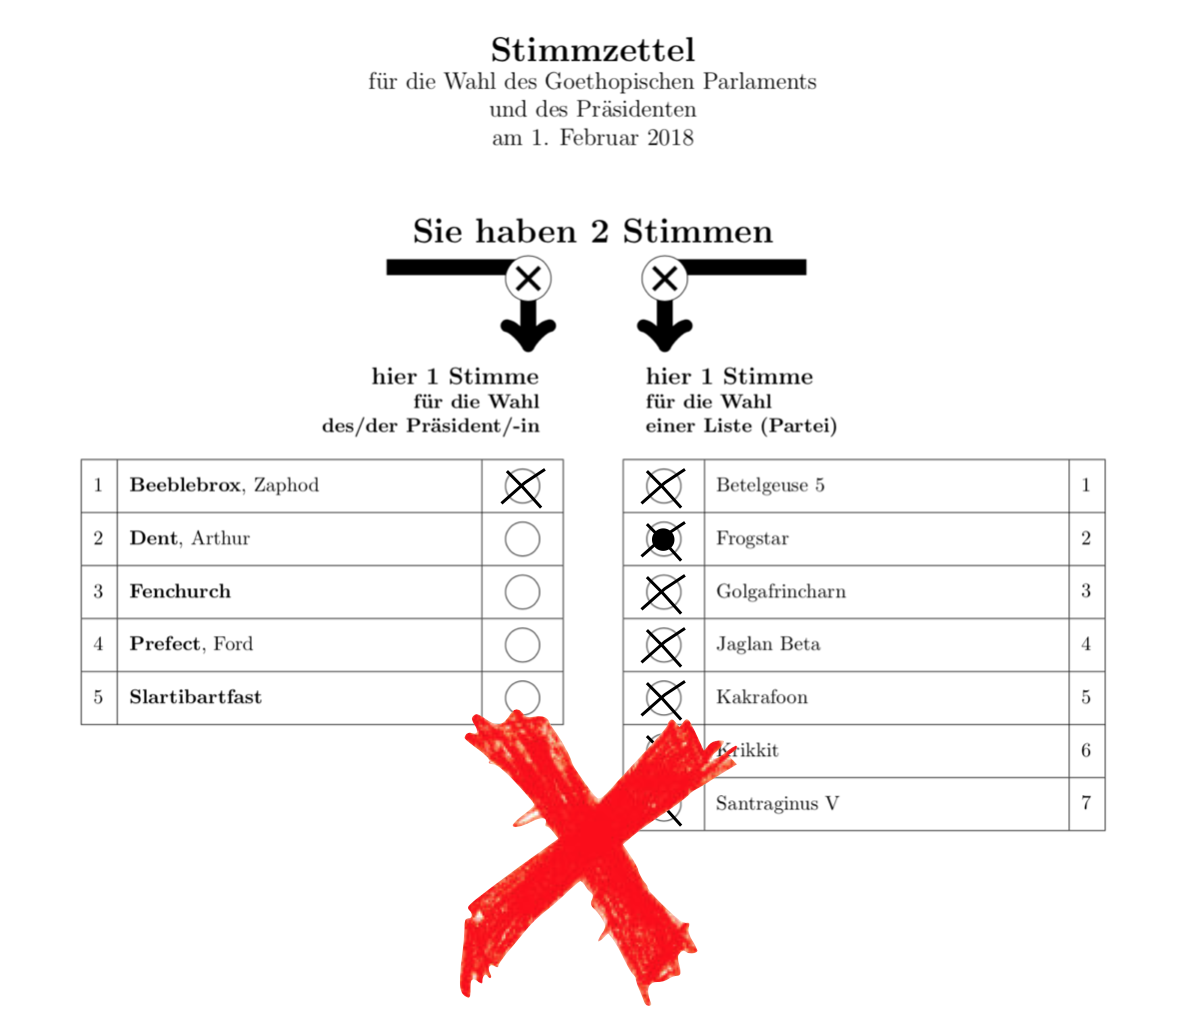
\includegraphics[width=\textwidth]{falsch_1.png}
    \end{minipage}
    \begin{minipage}{0.5\linewidth}
    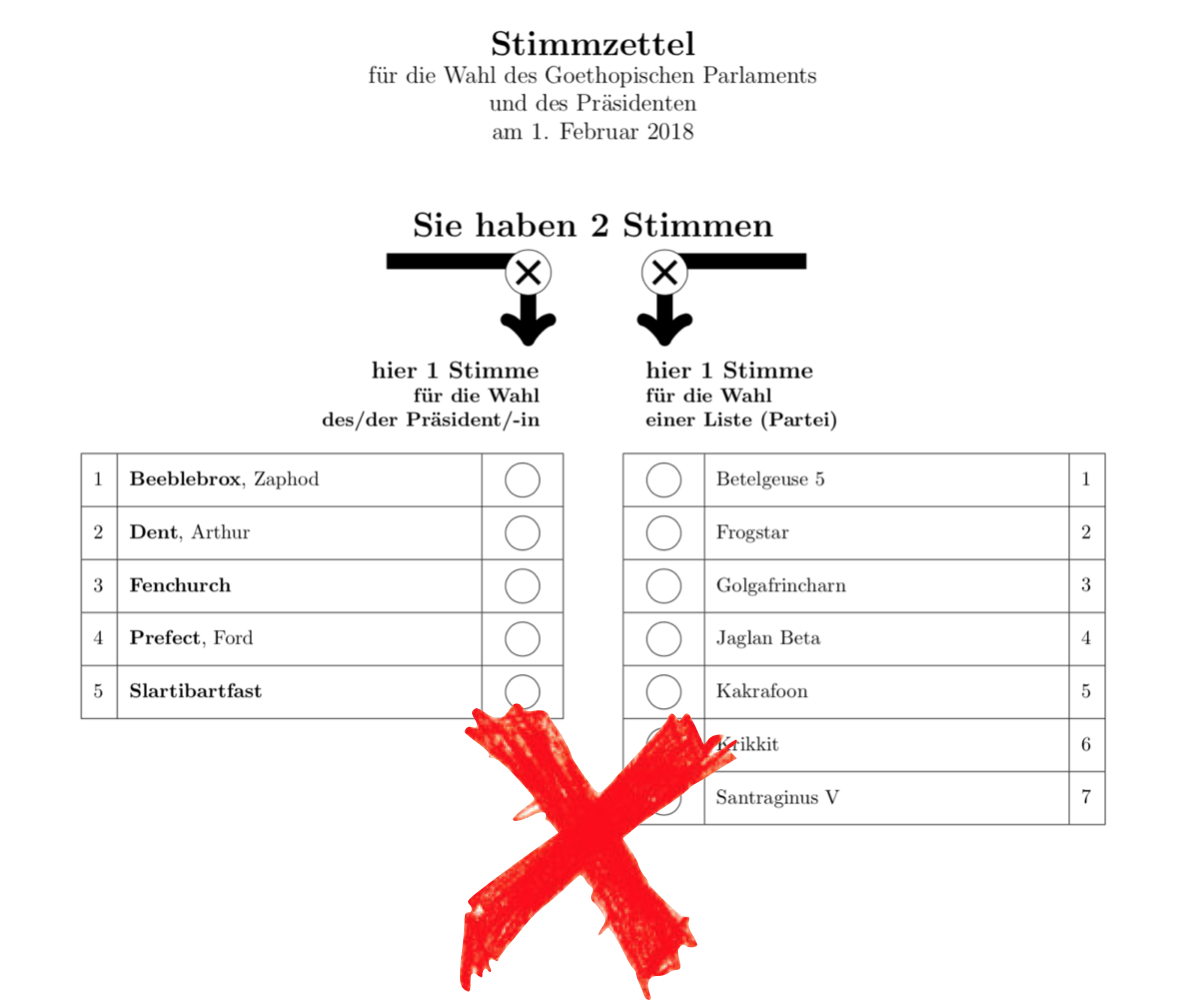
\includegraphics[width=\textwidth]{falsch_2.png}
    \end{minipage}
    \begin{minipage}{0.5\linewidth}
    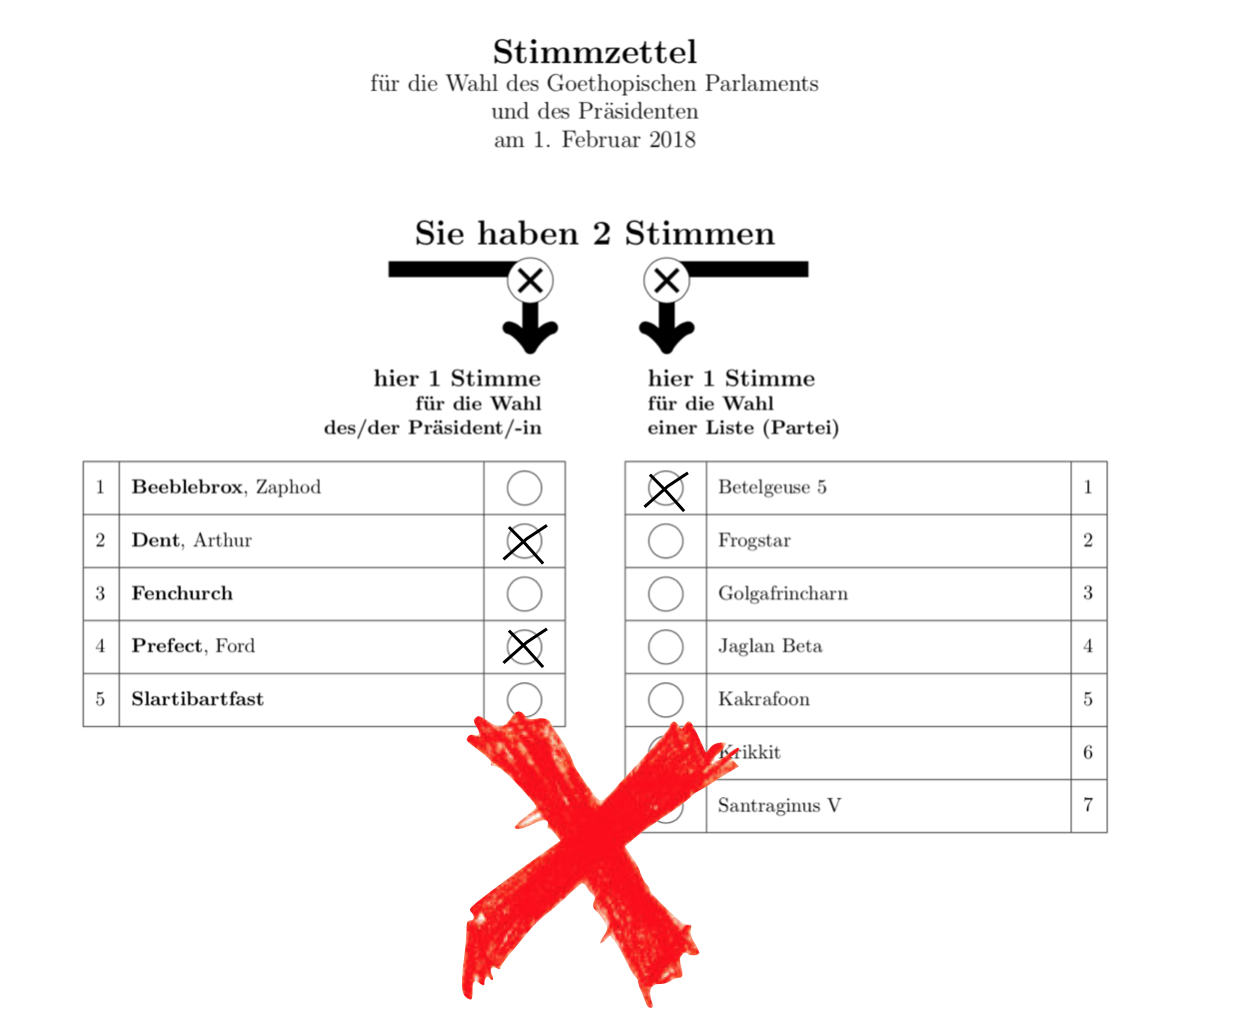
\includegraphics[width=\textwidth]{falsch_3.png}
    \end{minipage}
    \begin{minipage}{0.5\linewidth}
    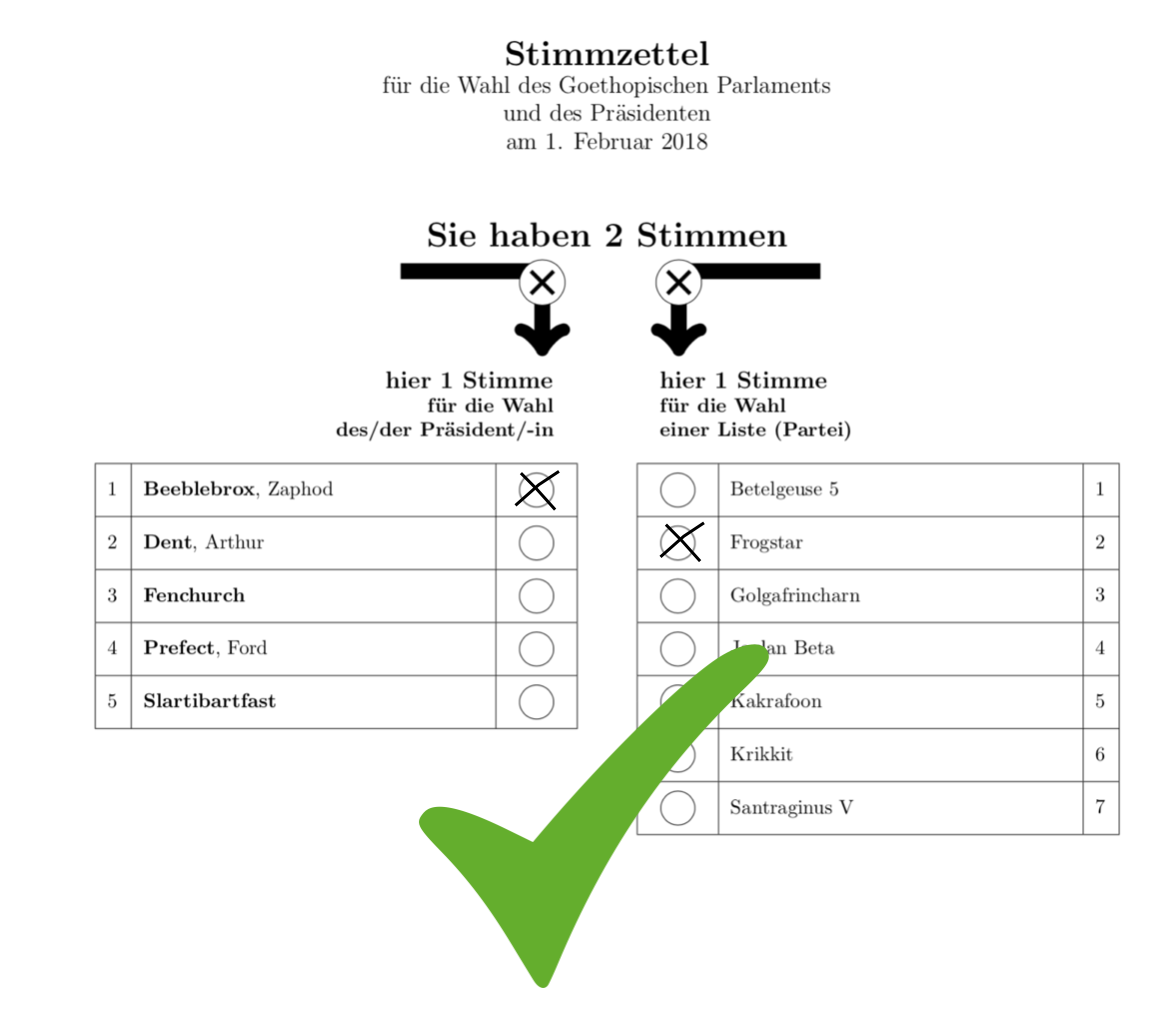
\includegraphics[width=\textwidth]{richtig.png}
    \end{minipage}

\topic{Nach der Wahl}

\begin{question}{Ab wann tagt das Parlament?}
    Sobald das endgültige Wahlergebnis veröffentlicht wurde, haben die Parteien Zeit, um eine Regierung zu bilden. 
    In der Woche vom 19.02. bis 23.02. muss die Präsidentin das Parlament das erste Mal einberufen, damit sich das Parlament konstituiert.
    Diese erste Sitzung wird als Tagesordnung vor allem formelle Aspekte wie Ratifizierung der Geschäftsordnung, Besetzung der Ministerien und Einstellungen wichtiger Beamten haben, 
    ab der zweiten Sitzung werden dann Gesetze erlassen und weitere Beamte eingestellt.
    \\
    \\
    Das Parlament entscheidet selber, wann es tagt, von der Häufigkeit der Parlamentssitzungen hängt allerdings der Erfolg des gesamten Projekts ab, deshalb
    ist das Parlament angehalten, wöchentlich zu tagen.
    
\end{question}
\begin{question}{Wie bewirbt man sich für einen Beamtenposten}
    Auf dieser Stellwand sind Vordrucke für Bewerbungen für einen Beamtenposten zu finden. Alternativ wird man sich auch auf der Website bewerben können.\\\\
    \textbf{Wichtig: Für Staatssekretärinnen, Richterinnen und Ministerinnen endet die Frist für Bewerbungen schon am 09.02.} \\\\Für die Bewerbungen ist Name und eine persönliche Motivation wichtig. Anhand der Motivation
    wählt das zuständige Ministerium aus den Bewerberinnen aus. \\
    Bei Richterinnen und Staatsanwältinnen kommt darüber hinaus noch die Teilnahme an einer Parlamentssitzung dazu, weil das Parlament die Beamten der Justiv einstellt.
\end{question}

\begin{question}{Welche Beamtenposten gibt es?}
\begin{itemize}
        \item Polizistinnen (12)
        \item Staatssekretärinnen (15)
        \item Straf- und Justizrichterinnen (3)
        \item Verfassungsrichterinnen (3)
        \item Staatsanwältin (1)
        \item Polizei-Chef (1)
        \item Zollbeamtinnen (12)
        \item Wirtschaftskontrolldienst-Mitarbeiterinnen (8)
    \end{itemize}
\end{question}

\begin{question}{Ab wann können Betriebe gegründet werden?}
    Ab frühestens 01.04. wird das Arbeitsministerium die Betriebsgründungen starten - dabei gilt das Prinzip \emph{first come, first serve}: 
    Falls ein Vorschlag schon schriftlich über die Website eingegangen ist, wird dem ersten Gründer natürlich der Vorzug gegeben.\\\\
    Das Arbeitsministerium wird an dieser Stelle in Zukunft noch weitere Informationen über Betriebsgründungen bekannt geben.
\end{question}

\section{Verfassungsänderungen}
Der kursiv-gesetzte Text zeigt jeweils eine Änderung zur vorherigen Fassung an. Diese Änderung wurde vom Organisations-Komittee von Schule als Staat mehrheitlich beschlossen.
    \setcounter{articleno}{18}
    \begin{article}[Wahlrecht]
        \setcounter{enumi}{5}
    \item \textit{Um die Wahlergebnisse optimal abzubilden, kann die Parlamentsgröße auf mindestens 27 bzw. maximal 35 Sitze verändert werden.}
    \end{article}
    \setcounter{articleno}{31}
    \begin{article}[Öffentlichkeit und Unabhängigkeit der Justiz]
    \item Alle 6 Beamtinnen der Justiz werden vom Parlament ins Amt gewählt und können vom Parlament mit einer \textit{3/4} Mehrheit entmachtet werden.
    \end{article}
\end{document}
